\documentclass{sig-alternate}

\clubpenalty=10000 
\widowpenalty=10000

\usepackage{color}
\usepackage{booktabs}
\usepackage{algorithm}
\usepackage{algorithmic}
\usepackage{graphicx}
\usepackage{xspace}
\usepackage{balance}
\usepackage{booktabs}
\usepackage{mathtools}
\usepackage{gensymb}


\def\TODO#1{\textcolor{red}{{\bf [TODO:}~#1{\bf ]}}}
\def\NOTE#1{\textcolor{blue}{{\bf [NOTE:}~#1{\bf ]}}}
\def\CHK#1 {\textcolor{magenta}{{\bf [CHK:}~#1{\bf ]}}}

\def\Vec#1{{\boldsymbol{#1}}}
\def\Mat#1{{\boldsymbol{#1}}}

\graphicspath{{./figures/}}

\newcommand{\fig}{{Figure}\@\xspace}
\newcommand{\tab}{{Table}\@\xspace}
\newcommand{\eqn}{{Equation}\@\xspace}
\newcommand{\ie}{{i.e.,}\@\xspace}
\newcommand{\eg}{{e.g.,}\@\xspace}
\newcommand{\etal}{{\it et~al.}\@\xspace}

\makeatletter
\DeclareRobustCommand{\etc}{%
    \@ifnextchar{.}%
        {etc}%
        {etc.\@\xspace}%
}
\makeatother

% 
%
%


%  
% front matter
%

% --- Author Metadata here ---
\conferenceinfo{MM}{'14 Orlando}
% \CopyrightYear{2007} % Allows default copyright year (20XX) to be over-ridden - IF NEED BE.
%\crdata{0-12345-67-8/90/01}  % Allows default copyright data (0-89791-88-6/97/05) to be over-ridden - IF NEED BE.
% --- End of Author Metadata ---


\title
  {
  Analyzing Video Lifelog in real-time
  }
  
% 
% 

\author
  {
  {Vu~Trang, Xudong~Shi}
  \\
  School of Computing, National University of Singapore, Singapore
  \\
  \\
  \{ xx, xudong.shi \}@nus.edu.sg
  }
% \numberofauthors{4}  
% \author
%   {
%   % 1st author
%   \alignauthor
%     Yongkang Wong\\
%     \affaddr{Interactive \& Digital Media Institute}\\
%     \affaddr{National University of Singapore}\\
%     \email{yongkang.wong@nus.edu.sg}
%   % 2nd author
%   \alignauthor
%     Name go here\ldots\\
%     \affaddr{xxx}\\
%     \affaddr{National University of Singapore}\\
%     \email{xxx@xxx.xxx}
%   \and
%   % 3rd author
%   \alignauthor
%     Name go here\ldots\\
%     \affaddr{xxx}\\
%     \affaddr{National University of Singapore}\\
%     \email{xxx@xxx.xxx}
%   % 4th author
%   \alignauthor
%     Mohan S Kankanhalli\\
%     \affaddr{School of Computing}\\
%     \affaddr{National University of Singapore}\\
%     \email{mohan@comp.nus.edu.sg}
%   }


% 
% 
% 


\begin{document}

\maketitle
\sloppy

%###############################################
\begin{abstract}
Video lifelog is becoming more and more popular. The amount of videos recorded
is rapidly increasing, however, applications that make use of these datas are
severly lacking. Current computer vision applications use a small number of
input images/videos because of the difficulty in aquiring computational
resources and storage options for large amounts of
data~\cite{2005_TSMC_Guo, 2010_KDD_White}. This work explores video lifelog
using big data framework. The works of image and video processing using big data
framework are provided as an overview of existing works in computer vision
community. We have proposed an approach for large scale video processing by
integrate video toolboxes and big data execution engine. As a case study, we
have implemented a people counting application and evaluated its acurracy and
efficiency. The evaluation shows that it can achieve good accuracy in feasible
execution time.

\end{abstract}


% http://www.acm.org/about/class/ccs98-html
% \category{I.2.10}{Vision and Scene Understanding}{Video analysis}
% \category{I.4.8}{Scene Analysis}{Motion}
\category{I.5.4}{Applications}{Signal processing}
\terms{Algorithms}
\keywords{Zero-Shot, Multi-Modality Mining, Instance Association}

%###############################################

\section{Introduction}
\label{sec:sec_intro}

The goal of lifelogging is to record and archive all information in one's life. 
This may include all texts, visual information, audio, media activity as well 
as biological data from sensors of one's body. The information would be archived
for the benefit of the lifelogger, and shared with others in various degrees as
controlled by him/her.  With the advances of technology, lifelog is becoming more
 and more popular. Fitness\footnote{http://www.fitbit.com/} tracker as one
 example is wildly worn by people to record  their sports activity, steps taken, distance traveled and calories
 burned.  Using this information, you can choose food, weight, and sleep
 tracking  to manage all aspects of your health.  At the same time, recent 
 technology has make wearable devices more accessible to common people. Google
 glass, and GoPro are just two brilliant example. With their support,  people
 are able to log their visual information.
Compares to other type of lifelog, vision-based lifelogs are more fruitful, and
if using properly, can help make people's life better. Recognizing objects of 
what people are watching can provide essential information about a person's 
activity and situation, thus have far-reaching impact on the application of 
vision in everyday life. The egocentric viewpoints from a wearable camera have
unique advantages in recognizing objects, such as a close view and seeing
objects in their natural positions.

With the vast amount of video and image collected daily, visual lifelog present 
challenges in analysis and store in a form with enable user to retrieved easily 
and extract useful information. Storing and managing videos are more challenging
than other types of data. Videos often followed some structure specification;
hence, prevent us from arbitrary reading and partitionning. Another challenge
is lacking of supported tools for large scale processing. Reseachers uses
special vision processing toolboxes when working with video. Unfortunately,
video processing is not well-supported by big data framework.

The goal of the project is an application that 
analyses vision-based lifelog video and enable user to retrieve in low
latency manner. In this project, we analyses and proposes an approach for using
big data framework in video processing. We also implement a PeopleCounting
application as a case study. Experiment result shows that our application
achieved good accuracy and promising performance with speedup of 5 comparing to
traditional approach - frame-base Matlab application.

This paper is organized as follows. Section 2 surveys related work on video
processing at large scale. Section 3 gives an overview of opportunities
and challenges when using big data framework for video processing. Section 4
describes our design of large scale video processing stack and our
implementation of PeopleCounting application as a case study. We evaluate
accuracy and efficiency of our implementation in Section 5, and conclude in
Section 6.

\section{Related Work}
\label{sec:sec_background}

\TODO{overview}
\TODO{image processing \& big data framework}
\TODO{video processing \ldots }
 
\section{Overview}
\label{sec:sec_theory}


\section{Implementation}
\label{sec:sec_algorithm}
\subsection{Architecture of Distributed Video Processing}

\subsubsection{Distributed Video Processing Software Stack}
Figure~\ref{fig:stack} shows the software stack for distributed video
processing.Similar to other types of big data application, data are also stored
in distributed file system such as Google File System (GFS)\cite{gfs}, Hadoop
Distributed File System (HDFS)\cite{hdfs}. However, storing video are more
challenged than storing text because its special structure does not allow
arbitrary partition and requires us to read sequentially.
\begin{figure}[htbp!]\centering
\vspace{-1ex}
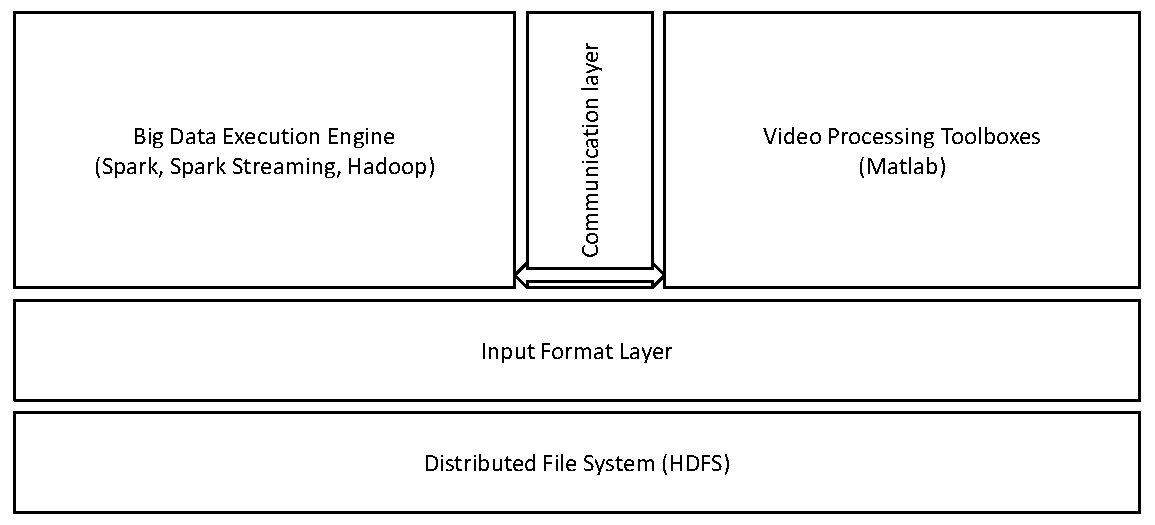
\includegraphics[width=0.5\textwidth]{figures/softwarestack.pdf}
\vspace{-4ex}
\caption{Distributed video processing software stack}
\label{fig:stack}
\end{figure}
 \textit{Input format
layer} is designed to efficiently partition, read and write large video files by
implementing distributed file systems APIs. One important aspect to be consider
when implement input format layer is storage unit and computation unit. As
mentioned earlier, we cannot arbitrary partition video into smaller blocks
(block size as partition metric). We have to decompress it and read as frames
which results in large numbers of smaller files and disk-consuming, before
processing. To overcome this problem, we decided to divide video into smaller
subvideos - also called \textit{Group-of-Picture (GOP)}, which will be describe
in Section~\ref{sec:gop}. 

At execution layer, we also use available big data execution engines such as
Spark\cite{spark}, Spark Streaming\cite{sparkstreaming}, Hadoop
MapReduce\cite{hadoop}. These execution engines are usually implemented in Java,
Scala which are not well-supported for video processing. We integrate the best
of both worlds in our design by leveraging well-supported video processing
ability of \textit{video processing toolboxes} and flexibility, scalability of
\textit{big data execution engines}. These two components communicate with each
other via a communication layer such as pipe, IPC protocol or memory-mapping which uses in our case study.

\subsubsection{Casestudy: Distributed People Counting in Large Video}
\TODO{problem statement}

Figure~\ref{fig:overview} shows execution process of our people counting
application. We use Spark as excution engine and Matlab as video processing
toolbox. Our application is implemented as a tradition MapReduce program with
one map and one reduce phase. During execution time, video stored in HDFS are read as GOPs by mappers. Since our processing logics are written in Matlab,
each mapper passes the GOP to a Matlab process via Spark \textit{pipe} methods.
This is an expensive call due to large overhead of Matlab startup. In our
implementation, we tried to minimize the number of Matlab call by processing at
coarse grain inputs - GOPs instead of frames. We also reduce Matlab startup
overhead by cross compile with MATLAB MCC (\textsection\ref{sec:mcc}).
\begin{figure}[htbp!]\centering
\vspace{-1ex}
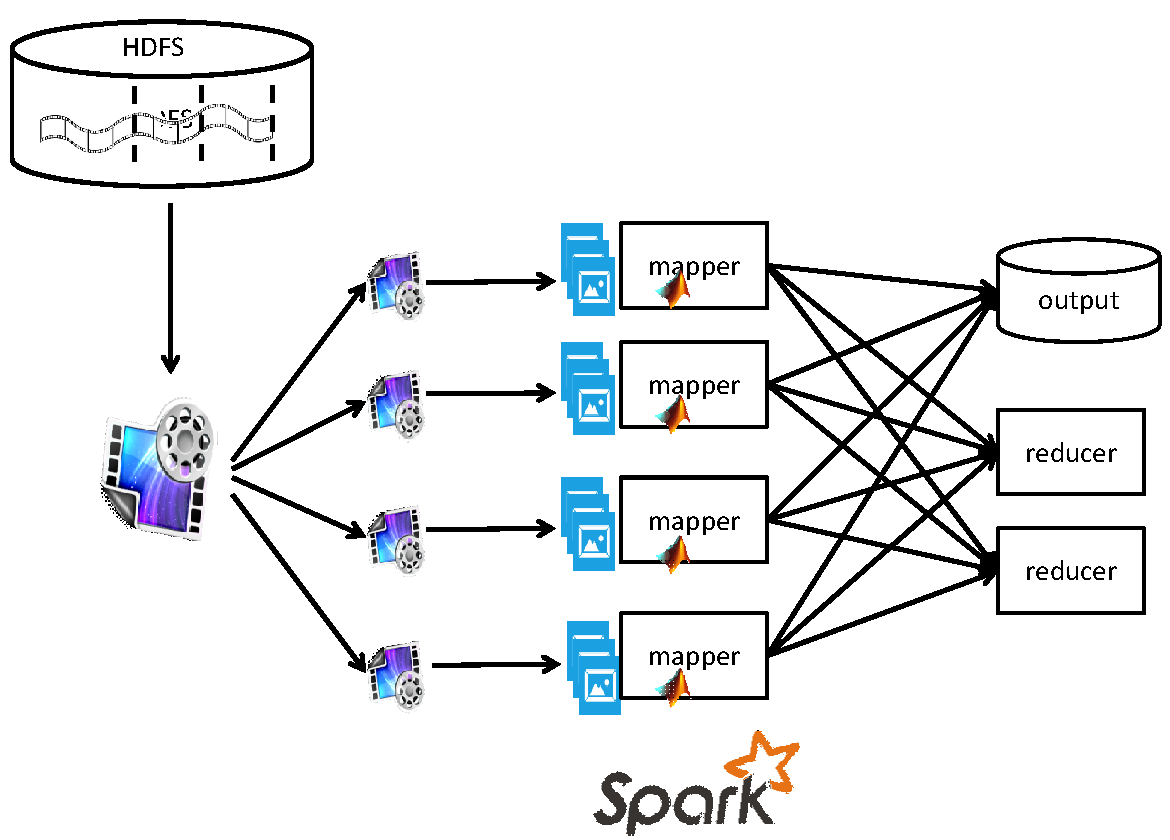
\includegraphics[width=0.5\textwidth]{figures/overview.pdf}
\vspace{-4ex}
\caption{Execution of people counting application}
\label{fig:overview}
\end{figure}

Each mapper takes an $<gop\_id, GOP>$ as input and return total number of people
appearance in that GOP as well as the bounding boxes and frame\_id they belong.
Mappers pass the result of number of people to reducer which will sum up for
final result. Bounding boxe details are stored back into HDFS for later
retrieval.

\subsection{Cross Compile with MATLAB MCC}\label{sec:mcc}
\subsubsection{Motivation}
The core functionality, person detection, is implemented in MATLAB language. It
is rather time consuming to call MATLAB scripts directly. The reason resides in 
the starting up time of MATLAB runtime. Since MATLAB is a scripting language, 
it requires an interpreter to parse the program line by line. A typical time 
spent on starting up MATLAB runtime would be 3-8 seconds, which cannot be
ignored for batch processing programs. Thus, we want to seek a way to reduce 
the starting up time for MATLAB runtime.

\subsubsection{What is MATLAB MCC}
MCC is the MATLAB command which stands for MATLAB Compiler. MCC prepares MATLAB 
files for deployment outside of the MATLAB runtime environment. It can generate 
wrapper files in C or C++, optionally build standalone binary files.
MCC command can be issued either from MATLAB command prompt (MATLAB terminal) or
the DOS or UNIX command line (Terminal). The resulting compiled files are
written  into current folder by default.
In summary, MATLAB MCC plays a role as a cross-platform compiler, which compiles
MATLAB scripts into C or C++ wrapper and binary executable. Finally, the binary 
executable has the same functionality as MATLAB script and is able to run without MATLAB runtime.

\subsubsection{Advantages}
The major advantage of using MATLAB MCC is shorter program running time. Since
we can execute the binary to accomplish the same task as MATLAB scripts, we
actually reduce the time of starting up MATLAB runtime environment.

\subsubsection{Usage}
The usage of MATLAB MCC mainly consists of two parts. 
Part I, compile MATLAB scripts \& produce binary executable: \\
mcc -mv -o binary\_execute  matlab\_script.m \\\\
Part II, execute binary from shell or other program: \\	
./binary\_execute.sh matlab\_path parameters


\subsection{Divide Video into GOP(Group of Pictures)} \label{sec:gop}
\subsubsection{Motivation}
We are utilizing Hadoop Distributed File System. We can not simply divide video
into frames, store all frames in Hadoop Distributed File System, carry out
person detection on each frame. This is due to the storage constrain and
processing granularity. On the one hand, it is storage inefficient to store all 
frames of a video. This is because no compression has been applied to the
redundant information of images. On the other hand, applying frame-based person 
detection is too granular. This will result in invoking external detection
procedure to frequently and enormous memory for storing image file metadata in 
namenode of Hadoop Distributed File System. Thus, there is emerging demand for 
establishing a method divide video into video clips (Group of Pictures) and
perform fragment-based person detection rather than frame-based person detection.

\subsubsection{Video Hierarchical Structure}
In order to increase random access, modern video compression standards all
support hierarchical video stream structure. Typical compression codecs are  
methods like MPEG-2, H264.

\begin{figure}[!htbp]
  \centering
  \begin{minipage}{1.0\columnwidth}
  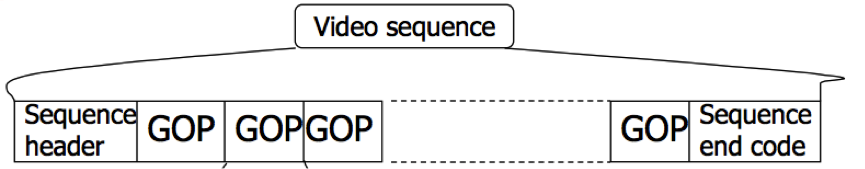
\includegraphics[width=1.05\linewidth]{video_gop}
  \end{minipage}
  
  \vspace{-1ex}
  \caption
    {
    \small
    The structure of a typical video sequence. There are many GoPs between video
    sequence header and sequence end code.}
  \label{fig:video_gop}
\end{figure}

As shown in~\fig\ref{fig:video_gop}, video sequence begins with a sequence
header and ends with a sequence end code. It is worth mentioning that there are
many GOPs (Group of Pictures) between sequence beginning and sequence ending 
position. One typical GoP may consists of 10 - 15 frames and is about 300 -
600KB large.
GOP is a independent unit which can be directly interpret by video player. We
can store multiple GoPs as a file in HDFS, and person detection can be done
based on those GoPs. However, the number of GoPs can be user-defined. Users can
use this parameter as one configuration to control the program granularity.

\begin{figure}[!htbp]
  \centering
  \begin{minipage}{1.0\columnwidth}
  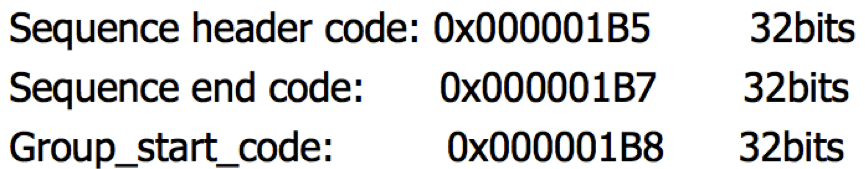
\includegraphics[width=1.05\linewidth]{video_gop_code}
  \end{minipage}
  
  \vspace{-1ex}
  \caption
    {
    \small
    Some typical location marker code in video. The video sequence header code,
    sequence end code and GoP start code. 
    }
  \label{fig:video_gop_code}
\end{figure}

The GoP location can be found by using GoP start code, typical GoP and video
sequence code are shown in~\fig\ref{fig:video_gop_code}. 


\subsubsection{Architecture of Distributed Video Processing}
\TODO{
Hi, can you add more for this part based on 
http://blog.pivotal.io/data-science-pivotal/products/using-hadoop-mapreduce-for-distributed-video-transcoding
}




\section{Experiment}
\label{sec:sec_experiment}

\subsection{Dataset}
In this paper, we use INRIA Dataset for model training and accuracy testing. 
The INRIA Dataset~\cite{2005_CVPR_Dalal} was collected under the project LEAR.
The INRIA Dataset contains 2666 color images, in which the author cropped 1774
images of humans from a varied set of personal photos settings. The cropped
images were normalized into size of 64 $\times$ 128 pixels. The people are
usually standing, but appear in any orientation and against a wide variety of 
background image including crowds. Many are bystanders taken from the image
backgrounds, so there is no particular bias on their poses. Negative images are
collected to contain a diverse of scenarios including indoor, outdoor, mountain,
city and beach scenes. Some images also focus on cars, bicycles, motorbikes,
furniture, \etc.
% add figure
Examples images are shown in~\fig\ref{fig:inria_dataset_example}.
INRIA Dataset also suffers from selection bias, because the manual selection of
images from photographs. It is worthwhile to mention that INRIA Datast has
fairly high resolution pedestrians, while most data sets gather from mobile
platform have median heights that ranges from 50 - 100
pixels~\cite{2012_PAMI_Dollar}. The INRIA Dataset helped driven the recent
advances of pedestrian detection. In spite of its limitations, it remains as one
of the most popular pedestrian detection data sets. 

\begin{figure*}[!t]
  \centering

	\begin{minipage}{2.0\columnwidth}
	  \begin{minipage}{0.1\columnwidth} \centerline{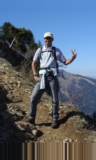
\includegraphics[width=1.05\linewidth]{inria_dataset/per00001}}  \end{minipage} \hfill 
	  \begin{minipage}{0.1\columnwidth} \centerline{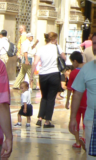
\includegraphics[width=1.05\linewidth]{inria_dataset/per00002}}  \end{minipage} \hfill 
	  \begin{minipage}{0.1\columnwidth} \centerline{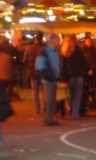
\includegraphics[width=1.05\linewidth]{inria_dataset/per000012}}  \end{minipage} \hfill 
	  \begin{minipage}{0.1\columnwidth} \centerline{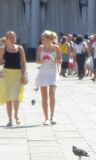
\includegraphics[width=1.05\linewidth]{inria_dataset/per00004}}  \end{minipage} \hfill 
	  \begin{minipage}{0.1\columnwidth} \centerline{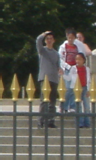
\includegraphics[width=1.05\linewidth]{inria_dataset/per00005}}  \end{minipage} \hfill 
	  \begin{minipage}{0.1\columnwidth} \centerline{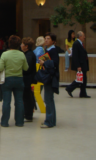
\includegraphics[width=1.05\linewidth]{inria_dataset/per00006}}  \end{minipage} \hfill 
	  \begin{minipage}{0.1\columnwidth} \centerline{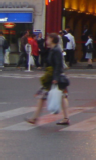
\includegraphics[width=1.05\linewidth]{inria_dataset/per00007}}  \end{minipage} \hfill 
	  \begin{minipage}{0.1\columnwidth} \centerline{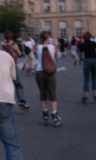
\includegraphics[width=1.05\linewidth]{inria_dataset/per00008}}  \end{minipage} \hfill 
	  \begin{minipage}{0.1\columnwidth} \centerline{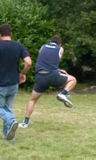
\includegraphics[width=1.05\linewidth]{inria_dataset/per00009}}  \end{minipage} \hfill
	\end{minipage}

    \begin{minipage}{2.0\columnwidth}
      \begin{minipage}{0.1\columnwidth} \centerline{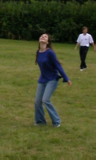
\includegraphics[width=1.05\linewidth]{inria_dataset/per000011}}  \end{minipage} \hfill 
      \begin{minipage}{0.1\columnwidth} \centerline{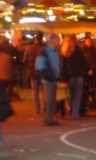
\includegraphics[width=1.05\linewidth]{inria_dataset/per000012}}  \end{minipage} \hfill 
      \begin{minipage}{0.1\columnwidth} \centerline{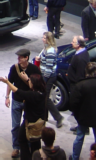
\includegraphics[width=1.05\linewidth]{inria_dataset/per000013}}  \end{minipage} \hfill 
      \begin{minipage}{0.1\columnwidth} \centerline{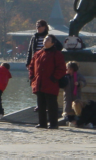
\includegraphics[width=1.05\linewidth]{inria_dataset/per000014}}  \end{minipage} \hfill 
      \begin{minipage}{0.1\columnwidth} \centerline{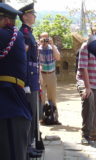
\includegraphics[width=1.05\linewidth]{inria_dataset/per000015}}  \end{minipage} \hfill 
      \begin{minipage}{0.1\columnwidth} \centerline{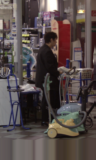
\includegraphics[width=1.05\linewidth]{inria_dataset/per000016}}  \end{minipage} \hfill 
      \begin{minipage}{0.1\columnwidth} \centerline{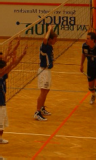
\includegraphics[width=1.05\linewidth]{inria_dataset/per000017}}  \end{minipage} \hfill 
      \begin{minipage}{0.1\columnwidth} \centerline{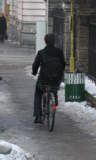
\includegraphics[width=1.05\linewidth]{inria_dataset/per000018}}  \end{minipage} \hfill 
      \begin{minipage}{0.1\columnwidth} \centerline{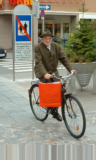
\includegraphics[width=1.05\linewidth]{inria_dataset/per000019}}  \end{minipage} \hfill
    \end{minipage}
    
  \vspace{-1ex}
  \caption
    {
    \small
	Some normalized image windows from the INRIA static person detection
	dataset. Note the variations in pose. Most of images contain people standing or
	walking. Some images have people running, going downhill, bicycling, or playing.
    }
  \label{fig:inria_dataset_example}
\end{figure*}


\subsection{Evaluation Method}
\label{subsec:evaluation_method}
The detection performance is measured by the number of true positive (TP - the
number of desired foreground objects detected by the detector) and false
positive  (FP - the number of background patches wrongly detected as the object
of  interest) detections~\cite{2013_ICCV_Hamed}. A detection is considered as
false positive if the predicted  bounding box with correlation response higher than the detection
threshold does not contain the target object. A detection is true positive if 
the overlap ratio $a_0$ between the predicted bounding box $B_p$ and a ground
truth bounding box $B_{gt}$ is more than a decision threshold $\theta$,
\begin{equation}
	a_0 = \frac{area(B_p \cap B_{gt})}{area(B_p \cup B_{gt})} \geq \theta
\end{equation}
The trade-off between TP and FP can be effectively measured using detection
rate versus false positive rate, Precision-Recall and Recall-FPPI  (false
positive per image) by varying a threshold and computing the recall and
precision/FPPI  for each threshold value, where
\begin{equation}
	Recall = \frac{TP}{nP}
\end{equation}

\begin{equation}
	Precision = \frac{TP}{TP + FP}
\end{equation}

\begin{equation}
	FPPI = \frac{FP}{N}
\end{equation}
where TP, nP, FP and N respectively indicate the true positive detections, the
total number of desired objects, the number of false detections and the number of test images.


\subsection{Experiment Accuracy Comparison}
The goal of experiment of accuracy comparison is to compare the performance of
person detection in standalone computer and computer clusters. In the
experiment, the person detector is trained using INRIA Dataset which is
described above. The testing data is also from from the same dataset which
consists of 288 images possible containing persons inside. 

After detection, we will get some bounding box locations for each image.
Combining detection results and ground truth information from INRIA Dataset.
We apply the evaluation in~\ref{subsec:evaluation_method} to get the
performance evaluation results. We plot the ROC(Receiver Operating
Characteristic) curve of the result.
The result is shown in~\fig\ref{fig:inria_roc}. As can be seen
in~\fig\ref{fig:inria_roc}, the detection result is same by performing HOG
method~\cite{2005_CVPR_Dalal} on standalone computer and computer clusters. The
slight different is result from some executing failure in the clusters. Thus
some testing images lack of the detection result. 

The result is of our expectation since we use same algorithm and also the same
implementation. The only difference is that the original implementation is
slightly modified so that it can be run on top of computer clusters to utilize
the computation power. 


\begin{figure}[!htbp]
  \centering
  \begin{minipage}{1.0\columnwidth}
  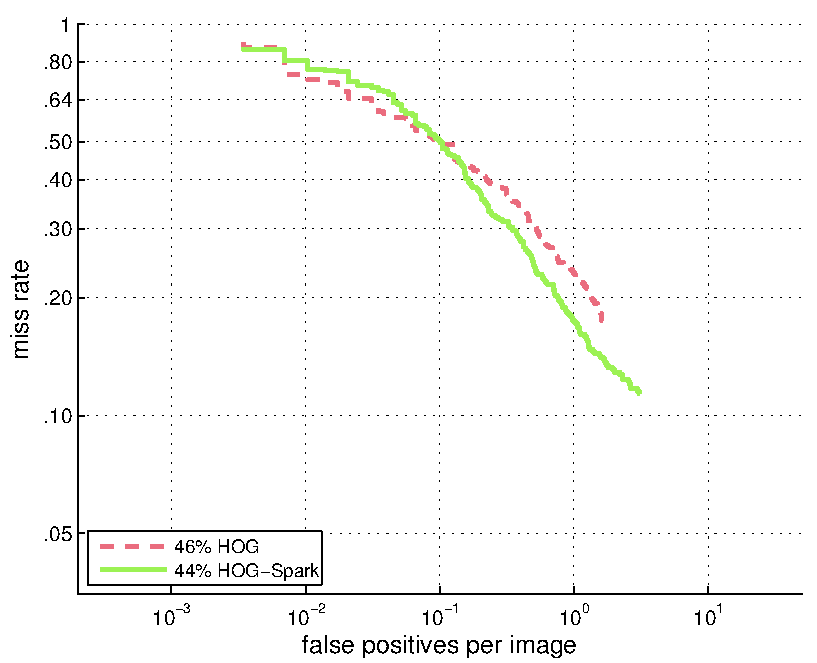
\includegraphics[width=1.05\linewidth]{InriaTest}
  \end{minipage}
  
  \vspace{-1ex}
  \caption
    {
    \small
	Results on INRIA Dataset with same detector running using standalone machine
	and computer clusters. The resulting performance is almost same as illustrated
	in the figure. }
  \label{fig:inria_roc}
\end{figure}



\section{Conclusion and Futurework}
\label{sec:sec_conclusion}

Conclusion go here\ldots

Futurework go here\ldots

% \section{Acknowledgement}
\label{sec:acknowledgement}

%% Full version
This research was carried out at the NUS-ZJU Sensor-Enhanced Social Media (SeSaMe) Centre. 
It is supported by the Singapore National Research Foundation under its International Research Centre @ 
Singapore Funding Initiative and administered by the Interactive Digital Media Programme Office.

% %% Space Limited version 
% This research was carried out at the SeSaMe Centre. 
% It is supported by the Singapore NRF under its IRC@SG Funding Initiative and administered by the IDMPO.

\balance
\bibliographystyle{abbrv}
\bibliography{reference}

\end{document}
